یک مثال ببینیم:

 فرض کنید که قرار است سیستم آموزشی یک دانشگاه را بنویسیم. یک کلاس student داریم.
  باید اطلاعات را جایی نگه داریم که persist شود. پس نمی‌شود در RAM نگه داریم. ساده‌ترین ایده‌ای که به ذهن می‌رسد،
   این است که مثلا ۸ بایت برای id، و برای اسم و فامیل هرکدام ۲۰ بایت.
    در مجموع ۴۸ بایت. در یک فایل به ازای هر ۴۸ بایت یک student داریم (پشت سر هم)
    .
    
    \begin{figure}[H]
        \centering
        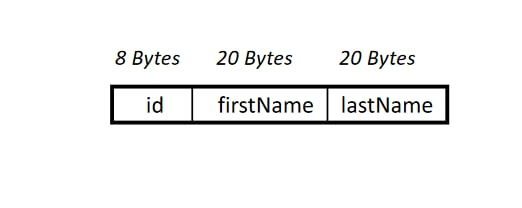
\includegraphics[width=0.7\textwidth]{source/stu1}
        \caption{قسمت های مختلف student}
    \end{figure}
    
    همچنین داریم به طور انتزاعی، فرض می‌کنیم که این فایل دنباله‌ای از record ها است.
    
    \begin{figure}[H]
        \centering
        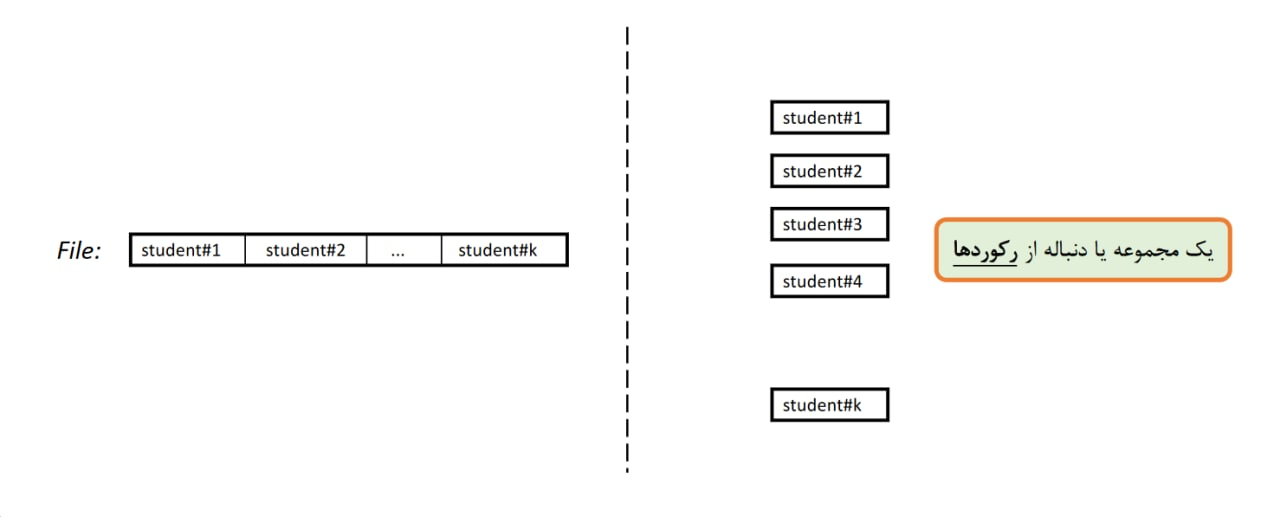
\includegraphics[width=0.7\textwidth]{source/stu2}
        \caption{انتزاع record}
    \end{figure}
    
    در اینجا مسائلی مشابه قبل پدید می‌آید. 
    به عنوان مثال حذف کردن یک 
    دانش‌آموز یک مسئله است (که می‌شود با ایده LinkedList این مسئله را حل کرد).
 یا مثلا فکر کنید که یک فیلد باید اضافه شود.
  در این صورت باید فایل باید مجددا ساختار دهی شود. که این کار راحتی نیست. 
 حال مثلا اگر یک ماهیت دیگر به اسم course اضافه کنیم،
  می‌دانیم که می‌توانیم با همان ایده‌ی قبلی این اطلاعات را ذخیره کنیم (یعنی چند بایت چند بایت ذخیره کنیم و قس علی هذا).
   دقت کنید که در اینجا فرقی اساسی بین Student و Course وجود ندارد و هرکدام میتواند یک رکورد باشد. بنابراین میتوانیم انتزاعی از یک Collection برای هرکدام از آنها در نظر بگیریم.
   
   \begin{figure}[H]
        \centering
        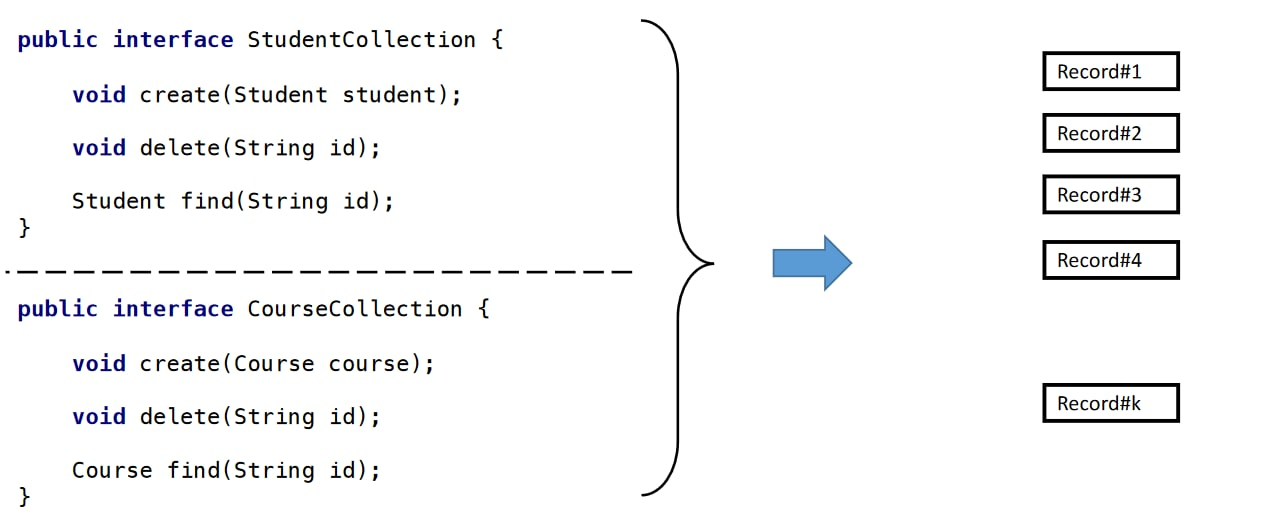
\includegraphics[width=0.7\textwidth]{source/stu3}
        \caption{انتزاع Record به صورت کلی‌تر}
    \end{figure}
   
 آیا مفهومی بین record و file وجود دارد؟ بله می شود مفهومی به صورت page تعریف کرد.
  می‌شود هر فایل را به صورت  chunk هایی دید که page نام دارند. مانند صفحات یک کتاب. انگار هر فایل یک مجموعه صفحه است.
  
  \begin{figure}[H]
        \centering
        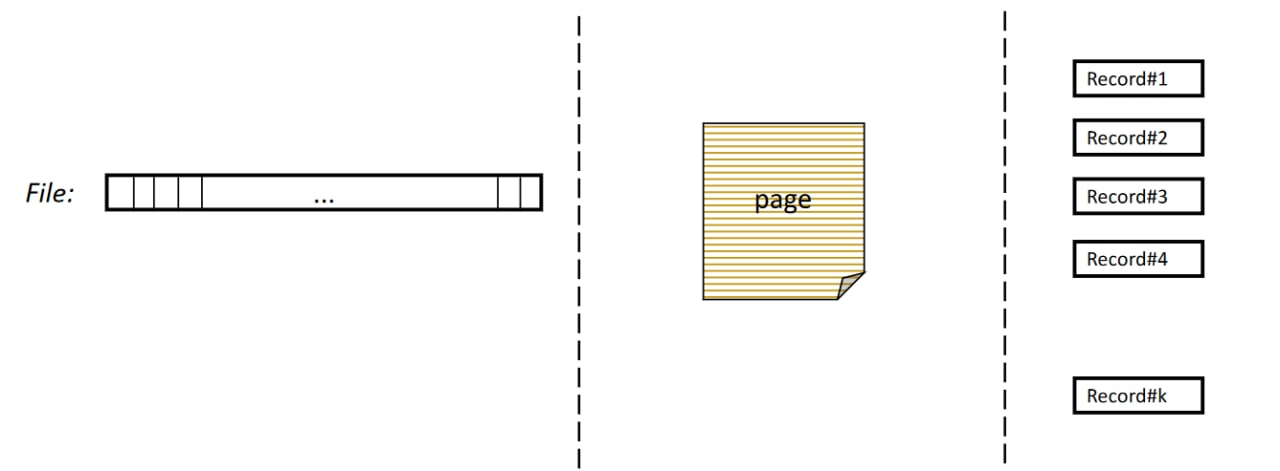
\includegraphics[width=0.7\textwidth]{source/stu4}
        \caption{انتزاع Page}
    \end{figure}
  
  تا یک زمانی برنامه نویس‌ها با مشی فایلینگ کار می‌کردند و دیتا را به صورت فایل ذخیره می‌کردند. این Approach مشکلاتی را به همراه دارد که چندتا از آنها عبارتند از:
  \begin{itemize}
      \item فایل‌ها چگونه ساماندهی شوند
      \item تغییر در داده‌ها چگونه اعمال شود
      \item چگونه میتوان بر روی داده‌ها جست و جوی سریع کرد
      \item مشکلات همروندی چگونه حل شوند
      \item از فایل ها چگونه بک‌آپ گرفته شود
      \item اگر داده‌ای خراب شد چگونه درست شود
  \end{itemize}
  
  تمام این دغدغه‌ها باعث این شد که یک مدل برای تبیین داده‌ها ساخته شود. مدل رابطه‌ای توسط Ted Codd در سال 1970 ساخته شد. این مدل یک انتزاع بر روی فایلینگ میباشد. این مدل از مفهوم ریاضی رابطه برای تبیین داده‌ها استفاده میکند.
  $$
  R \subset D_1\times\dots\times D_n
  $$